\documentclass[12pt]{amsart}

\addtolength{\hoffset}{-2.25cm}
\addtolength{\textwidth}{4.5cm}
\addtolength{\voffset}{-2.5cm}
\addtolength{\textheight}{5cm}
\setlength{\parskip}{0pt}
\setlength{\parindent}{15pt}
\usepackage{listings}
\usepackage{amsthm}
\usepackage{amsmath}
\usepackage[spanish]{babel}
\usepackage[sort&compress, numbers]{natbib}
\usepackage{amssymb}
\usepackage[utf8]{inputenc}
\usepackage[colorlinks = true, linkcolor = thistle, citecolor = thistle, final]{hyperref}
\usepackage{listings}
\usepackage{ragged2e}
\usepackage{subcaption} 
\usepackage{minted}
\usemintedstyle{borland}
\usepackage{multicol}
\usepackage{listings}
\usepackage{xcolor}
\usepackage{graphicx}
\usepackage[sort&compress, numbers]{natbib}
\usepackage{xcolor}
\usepackage{listings}
\usepackage{ragged2e}
\usepackage{graphicx}
\usepackage[sort&compress, numbers]{natbib}
\usepackage{xcolor}
\usepackage{listings}
\usepackage{ragged2e}
\hypersetup{
    colorlinks=true,
    linkcolor=violet,
    filecolor=violet,     
    urlcolor=violet,
    citecolor=violet,
}
\usepackage{graphicx}
\usepackage[sort&compress, numbers]{natbib}
\usepackage{xcolor}
\usepackage{listings}
\usepackage{ragged2e}

\lstset{style=mystyle}
\usepackage{graphicx}
\usepackage{multicol}
\usepackage{ marvosym }
\newcommand{\ds}{\displaystyle}


\pagestyle{myheadings}

\setlength{\parindent}{0in}
\begin{document}

\pagestyle{empty}



\thispagestyle{empty}

{\scshape Simulación} \hfill  \hfill  {\scshape 28/Abr/2021}

\begin{center}
   \maketitle {\scshape \Large Tarea 9: Interacciones entre partículas}
\end{center}
\begin{center}
    \maketitle\author{C. María Montemayor Palos}
\end{center}
\maketitle

\hrule
\hrule
\bigskip
\section{Objetivo}
Agregar a cada partícula una masa y que cause fuerzas gravitacionales (atracciones) además de las fuerzas causadas por las cargas. Graficar la relación entre los tres factores: la velocidad, la magnitud de la carga, y la masa de las partículas.


\section{Metodología}
Para efectos de la tarea \cite{dra} se utiliza el programa R versión 4.0.4 \cite{R} para Windows. Se consideran los parámetros de $n$= 50 partículas, normalizando $x$ y $y$ de 0 a 1 y $c$ entre -1 y 1.

\section{Código}
Se modifica el código de Schaeffer \cite{codigo} añadiendo una masa en el \texttt{data.frame} que sea capaz de generar fuerzas gravitacionales.
\renewcommand{\listingscaption}{Código}
\begin{listing}[H]
  \begin{minted}[linenos,mathescape,texcl]{clojure}
n <- 50
p <- data.frame(x = rnorm(n), y=rnorm(n), c=rnorm(n), m=rnorm(n))
  \end{minted}
  \label{codigo1}
\end{listing}

Se observa que en el código original la nueva posición de la partícula es dictada por la magnitud de la fuerza resultante entre una partícula y las demás, es decir a mayor magnitud de fuerza, mayor será el desplazamiento. Es por ello que se incluye la masa.
\renewcommand{\listingscaption}{Código}
\begin{listing}[H]
  \begin{minted}[linenos,mathescape,texcl]{clojure}
xmax <- max(p$x)
xmin <- min(p$x)
p$x <- (p$x - xmin) / (xmax - xmin) # ahora son de 0 a 1
ymax <- max(p$y)
ymin <- min(p$y)
p$y <- (p$y - ymin) / (ymax - ymin) # las y tambien
cmax <- max(p$c)
cmin <- min(p$c)
p$c <- 2 * (p$c - cmin) / (cmax - cmin) - 1 # cargas son entre -1 y 1
p$g <- round(5 * p$c) # coloreamos segun la carga a 11 niveles de -5 a 5
mmax=max(p$m)
mmin=min(p$m)
p$m=(p$m-mmin)/(mmax-mmin) + 0.1
  \end{minted}
  \label{codigo1}
\end{listing}
\clearpage
Se incluye la masa \texttt{m} como divisor de la fuerza en función a esta masa.
\renewcommand{\listingscaption}{Código}
\begin{listing}[H]
  \begin{minted}[linenos,mathescape,texcl]{clojure}
  for (j in 1:n) {
    cj <- p[j,]$c
    dir <- (-1)^(1 + 1 * (ci * cj < 0))
    dx <- xi - p[j,]$x
    dy <- yi - p[j,]$y
    factor <- dir * abs(ci - cj) / (sqrt(dx^2 + dy^2) + eps)
    fx <- fx - dx * factor
    fy <- fy - dy * factor
  }
  return(c(fx, fy)/(mi))
  \end{minted}
  \label{codigo1}
\end{listing}

\section{Resultados y discusión}
En la figura \ref{fig1} se presentan las posiciones de las partículas generadas en cuatro pasos a lo largo del proceso de interacción entre ellas, en donde se sitúan inicialmente al azar, conforme pasan las iteraciones se logra apreciar como las partículas se aglomeran debido a las fuerzas de atracción entre estas. Se puede encontrar el gif generado del movimiento de las partículas en el repositorio de \cite{mtyor}.

\begin{figure}[h!]
\centering
\begin{subfigure}[b]{0.3\linewidth}
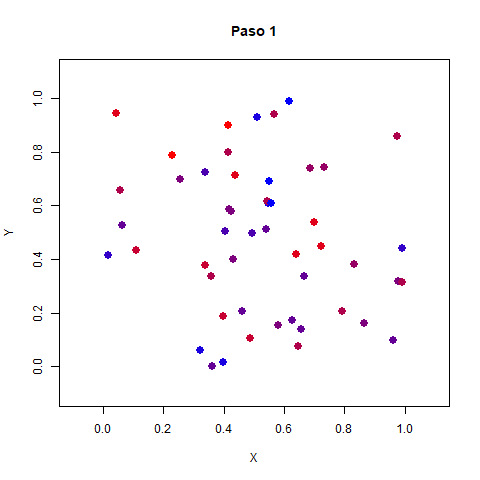
\includegraphics[width=\linewidth]{t9_t01.png}
\caption{Paso 1.}
\label{a}
\end{subfigure}
\begin{subfigure}[b]{0.3\linewidth}
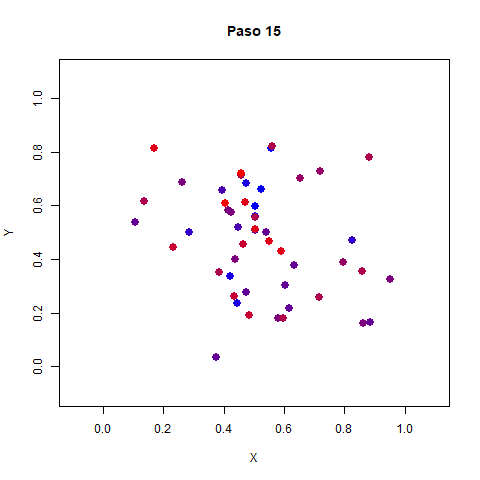
\includegraphics[width=\linewidth]{t9_t15.png}
\caption{Paso 15.}
\label{b}
\end{subfigure}
\begin{subfigure}[b]{0.3\linewidth}
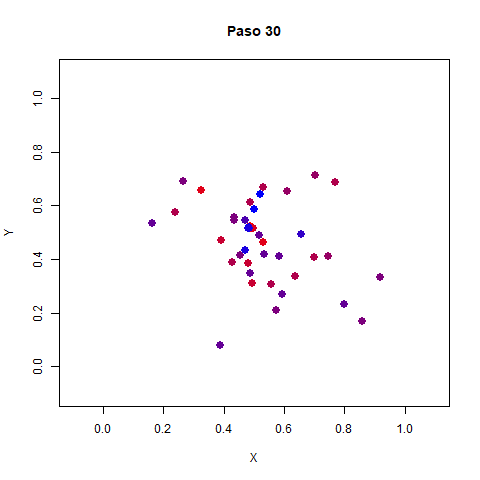
\includegraphics[width=\linewidth]{t9_t30.png}
\caption{Paso 30.}
\label{c}
\end{subfigure}
\begin{subfigure}[b]{0.3\linewidth}
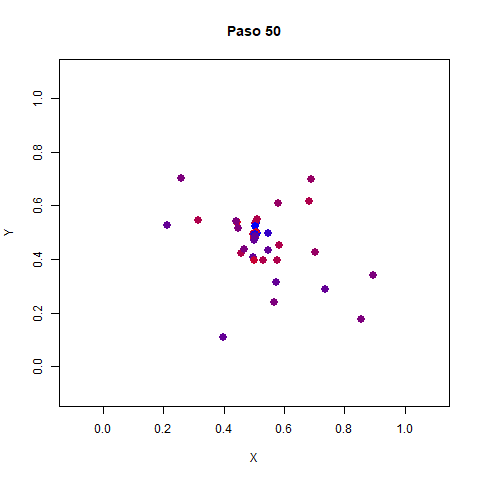
\includegraphics[width=\linewidth]{t9_t50.png}
\caption{Paso 50.}
\label{d}
\end{subfigure}
\caption{Movimiento de las partículas en relación a su velocidad, carga y masa.}
\label{fig1}
\end{figure}

\clearpage

Se genera un diagrama ternario (figura \ref{fig2}) para observar mejor de manera visual el comportamiento de las partículas en relación a su masa, velocidad y carga, correspondiendo al color morado una masa mayor y el color rosa una masa menor.
\begin{figure} [h!]
    \centering
    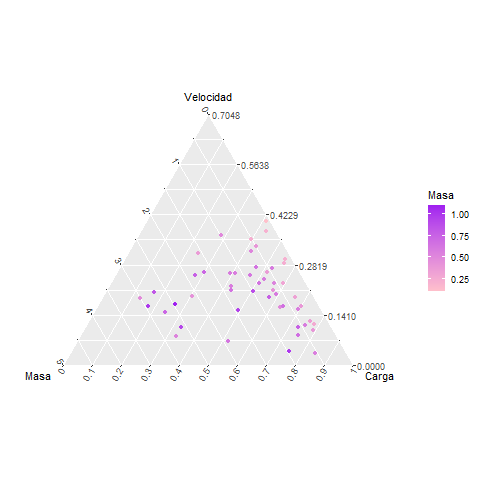
\includegraphics[width=0.6\textwidth]{DiagramaTernario.png}
    \caption{Diagrama ternario en relación a la masa, velocidad y carga de las partículas.}
    \label{fig2}
\end{figure}


\section{Conclusión}
En conclusión como se puede apreciar en la figura \ref{fig2} las partículas con una mayor masa afecta directamente a su velocidad disminuyéndola, por lo tanto a menor masa, mayor velocidad. También se observa que existe una mayor velocidad para aquellas partículas que tienen mayor carga, pero aún así se ven afectadas por la masa.

\clearpage
\bibliography{referencias}
\bibliographystyle{plainnat}


\end{document}
